% !TEX root = ../main.tex

\section{Функції кількох випадкових аргументів}
\subsection{Випадок довільної функції}
Нехай $\varphi : \mathbb{R}^n \to \mathbb{R}$ --- задана числова функція.

Якщо $\vec{\xi} = \left(\xi_1, ..., \xi_n\right)$ --- дискретний випадковий вектор, тоді $\eta = \varphi(\vec{\xi})$ --- ДВВ.
Побудову закону розподілу $\eta$ доцільно розглянути на прикладі.
\begin{example}
    $\vec{\xi} = \left( \xi_1, \xi_2\right)$ задано таблицею розподілу:
    \begin{tabular}{|c|c|c|c|}
        \hline
        \diagbox{$\xi_2$}{$\xi_1$} & $0$ & $1$ & $2$ \\
        \hline
        $-1$ & $0.1$ & $0.2$ & $0.3$ \\
        \hline
        $1$ & $0.2$ & $0.1$ & $0.1$ \\
        \hline
    \end{tabular}.

    \noindentЗнайти закони розподілу $\eta_1 = \xi_1 \xi_2$ та $\eta_2 = \xi_1 + \xi_2$.
    Для цього треба визначити значення, які приймають ці величини, та обчислити відповідні ймовірності.
    
    $\eta_1$ приймає значення $-2$ (коли $\xi_1 = 2$, $\xi_2 = -1$), 
    $-1$ (коли $\xi_1 = 1$, $\xi_2 = -1$), 
    $0$ (коли $\xi_1 = 0$, $\xi_2 = -1$ або $\xi_2 = 1$), 
    $1$ (коли $\xi_1 = 1$, $\xi_2 = 1$), 
    $2$ (коли $\xi_1 = 2$, $\xi_2 = 1$).

    $\eta_2$ приймає значення $-1$ (коли $\xi_1 = 0$, $\xi_2 = -1$), 
    $0$ (коли $\xi_1 = 1$, $\xi_2 = -1$), 
    $1$ (коли $\xi_1 = 0$, $\xi_2 = 1$ або $\xi_1 = 2$, $\xi_2 = -1$), 
    $2$ (коли $\xi_1 = 1$, $\xi_2 = 1$), 
    $3$ (коли $\xi_1 = 2$, $\xi_2 = 1$).
    Відповідні сумісні ймовірності отримуємо з таблиці з таблиці розподілу $\vec{\xi}$.

    \begin{tabular}{|c|c|c|c|c|c|}
        \hline
        $\eta_1$ & $-2$ & $-1$ & $0$ & $1$ & $2$ \\
        \hline
        $p$ & $0.3$ & $0.2$ & $0.3$ & $0.1$ & $0.1$ \\
        \hline
    \end{tabular}
    \begin{tabular}{|c|c|c|c|c|c|}
        \hline
        $\eta_2$ & $-1$ & $0$ & $1$ & $2$ & $3$ \\
        \hline
        $p$ & $0.1$ & $0.2$ & $0.5$ & $0.1$ & $0.1$ \\
        \hline
    \end{tabular}
\end{example}

Якщо $\vec{\xi} = \left(\xi_1, ..., \xi_n\right)$ --- неперервний випадковий вектор
із щільністю $f_{\vec{\xi}} (\vec{x})$, то можна знайти функцію розподілу $\eta = \varphi(\vec{\xi})$.
$$F_\eta (y) = P \left\{ \eta < y\right\} = P \left\{ \xi \in D_y\right\} = \underset{D_y}{\int ... \int} f_{\vec{\xi}} (\vec{x}) d \vec{x}, \text{ де }D_y = \left\{\vec{x} \in \mathbb{R}^n : \varphi(\vec{x}) < y\right\}$$

Розглянемо тепер взаємно однозначне гладке перетворення $\vec{\psi} : \mathbb{R}^n \to \mathbb{R}^n$ та
знайдемо щільність розподілу $\vec{\eta} = \vec{\psi} (\vec{\xi})$. Для множини $D \subset \mathbb{R}^n$
$P\left\{ \vec{\psi} (\vec{\xi}) \in D\right\} = P\left\{ \vec{\xi} \in \vec{\psi}^{-1}(D)\right\} = \int_{\vec{\psi}^{-1}(D)} f_{\vec{\xi}} (\vec{x}) d\vec{x} = 
\left[ \text{заміна }\vec{y} = \vec{\psi}(\vec{x})\right] = \int_D f_{\vec{\xi}} (\vec{\psi}^{-1}(\vec{y})) \left| \mathcal{J}^{-1} (\vec{\psi}^{-1}(\vec{y})\right| d\vec{y}$,
де $\mathcal{J} (\vec{x})$ --- якобіан $\vec{\psi}$. Отже,
$$f_{\vec{\eta}} (\vec{y}) = f_{\vec{\xi}} (\vec{\psi}^{-1}(\vec{y})) \left| \mathcal{J}^{-1} (\vec{\psi}^{-1}(\vec{y})\right|$$

\begin{example}
    Нехай $A$ --- невироджена матриця розміру $n \times n$, $\vec{b} \in \mathbb{R}^n$ --- деякий вектор, $\vec{\xi}$ --- неперервний випадковий вектор.
    Знайти щільність розподілу $\vec{\eta} = A \vec{\xi} + \vec{b}$.

    Тут $\vec{y} = \vec{\psi}(\vec{x}) = A \vec{x} + \vec{b}$, тому $\vec{\psi}^{-1} (\vec{y}) = A^{-1} (\vec{y} - \vec{b})$. Якобіан $\vec{\psi}$ рівний $\left| \det A\right|$. 
    Отже,
    $f_{\vec{\eta}}(\vec{y}) = \frac{1}{\left| \det A\right|} f_{\vec{\xi}}\left(A^{-1} (\vec{y} - \vec{b})\right)$
\end{example}

\subsection{Закон розподілу мінімуму та максимуму}

Нехай $\xi_1, ..., \xi_n$ незалежні та розподілені однаково, як деяка випадкова величина $\xi$.
Знайдемо розподіл їх мінімуму та максимуму.
\begin{enumerate}
    \item $\mu_1 = \min\left\{\xi_1, \xi_2, ..., \xi_n\right\}$.

    $F_{\mu_1} (x) = P \left\{ \min\{\xi_1, \xi_2, ..., \xi_n\} < x \right\} =
    1 - P \left\{ \min\{\xi_1, \xi_2, ..., \xi_n\} \geq x \right\} =$

    $ = 1 - P \left\{ \xi_1 \geq x, \xi_2 \geq x, ..., \xi_n \geq x \right\} = 
    1 - P\left\{ \xi_1 \geq x\right\} \cdot P\left\{ \xi_2 \geq x\right\} \cdot ... \cdot P\left\{ \xi_n \geq x\right\} = $
    
    $ = 1 - (P\left\{ \xi \geq x\right\})^n = 1 - (1- F_\xi (x))^n$.

    Якщо $\xi_1, ..., \xi_n$ --- неперервні, то $f_{\mu_1} (x) = \left( F_{\mu_1} (x)\right)^\prime = n (1- F_\xi (x))^{n-1} f_\xi(x)$.
    \item $\mu_2 = \max\left\{\xi_1, \xi_2, ..., \xi_n\right\}$.

    $F_{\mu_2} (x) = P \left\{ \max\{\xi_1, \xi_2, ..., \xi_n\} < x \right\} =
    P \left\{ \xi_1 < x, \xi_2 < x, ..., \xi_n < x \right\} = $

    $ = P\left\{ \xi_1 < x\right\} \cdot P\left\{ \xi_2 < x\right\} \cdot ... \cdot P\left\{ \xi_n < x\right\} =
    (P\left\{ \xi < x\right\})^n = (F_\xi (x))^n$.

    Якщо $\xi_1, ..., \xi_n$ --- неперервні, то $f_{\mu_2} (x) = \left( F_{\mu_2} (x)\right)^\prime = n (F_\xi (x))^{n-1} f_\xi(x)$.
\end{enumerate}

\begin{example}
    Нехай $\xi_1, ..., \xi_n$ незалежні та мають розподіл $\mathrm{Exp}(\lambda)$. Знайти розподіл їх мінімуму.

    \noindent$f_{\min}(x) = n (1-(1-e^{-\lambda x}))^{n-1} \lambda e^{-\lambda x} = n \lambda e^{-n\lambda}$ при $x \geq 0$ та $0$ при $x < 0$.
    
    \noindentОтже, $\min\{\xi_1, ..., \xi_n\} \sim \mathrm{Exp} (n \lambda)$.
\end{example}

\subsection{Закон розподілу добутку двох НВВ}
Нехай маємо $\vec{\xi} = (\xi_1, \xi_2)^T$ --- неперервний випадковий вектор та
$f_{\xi_1 \xi_2}(x, y)$ відома.

\noindent\textbf{Задача}: знайти розподіл $\eta = \xi_1\xi_2$.

Розпишемо функцію розподілу за вже відомою схемою:

$F_\eta(z) = \iint\limits_{D_z}f_{\xi_1\xi_2}(x, y)dxdy$, $D_z = \left\{(x, y)^T \in 
\mathbb{R}^2 : xy < z\right\}$

\underline{Розглянемо два варіанти:}
\begin{enumerate}[label=\Roman*)]
    \item 
\begin{tabular}{c p{8.8cm}}
    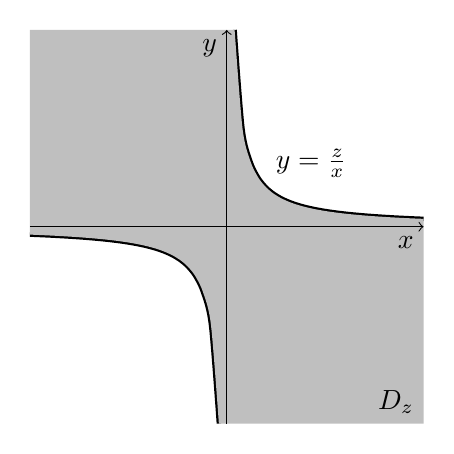
\begin{tikzpicture}[baseline={(current bounding box.north)} ,scale = 0.5]
        \draw [domain=0.2:5, smooth, variable = \x, ultra thick] plot ({\x}, 
        {
            1/\x
        });
        \fill [lightgray, domain=0.2:5, smooth, variable = \x] plot ({\x}, 
        {
            1/\x
        }) -- (5, -5) -- (0, -5) -- (0, 5) -- (0.2, 5);
        \draw [domain=-5:-0.2, smooth, variable = \x, ultra thick] plot ({\x}, 
        {
            1/\x
        });
        \fill [lightgray, domain=-5:-0.2, smooth, variable = \x] plot ({\x}, 
        {
            1/\x
        }) -- (0, -5) -- (0, 5) -- (-5, 5) -- (-5, -0.2);
        \draw [->] (-5, 0) -- (5, 0);
        \draw [->] (0, -5) -- (0, 5);
        \node [below left] at (5, 0) {$x$};
        \node [below left] at (0, 5) {$y$};
        \node [above left] at (5, -5) {$D_z$};
        \node [above right] at (1, 1) {$y = \frac{z}{x}$};
    \end{tikzpicture} &
    \underline{$z > 0$ : $y = \frac{z}{x}$}

    $x > 0$ : $y < \frac{z}{x}$
    
    $x < 0$ : $y > \frac{z}{x}$

    $F_\eta (z) = \int\limits^{0}_{-\infty}dx\int\limits_{\frac{z}{x}}^{+\infty}
    f_{\vec{\xi}}(x, y) dy + \int\limits_0^{+\infty}dx\int\limits_{-\infty}^{\frac{z}{x}} 
    f_{\vec{\xi}}(x, y) dy$

    Продиференціюємо обидві частини по $z$:

    $f_\eta(z) = -\int\limits_{-\infty}^0 \frac{1}{x}f_{\vec{\xi}}(x, \frac{z}{x})dx + 
    \int\limits_0^{+\infty}\frac{1}{x}f_{\vec{\xi}}(x, \frac{z}{x})dx$
\end{tabular}

\item
\begin{tabular}{c p{8.8cm}}
    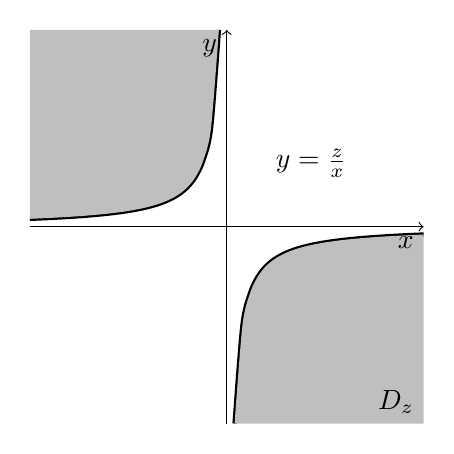
\begin{tikzpicture}[baseline={(current bounding box.north)} ,scale = 0.5]
        \draw [domain=0.2:5, smooth, variable = \x, ultra thick] plot ({\x}, 
        {
            -1/\x
        });
        \fill [lightgray, domain=0.2:5, smooth, variable = \x] plot ({\x}, 
        {
            -1/\x
        }) -- (5, -5) -- (0.2, -5);
        \draw [domain=-5:-0.2, smooth, variable = \x, ultra thick] plot ({\x}, 
        {
            -1/\x
        });
        \fill [lightgray, domain=-5:-0.2, smooth, variable = \x] plot ({\x}, 
        {
            -1/\x
        }) -- (-5, 5) -- (-5, 0.2);
        \draw [->] (-5, 0) -- (5, 0);
        \draw [->] (0, -5) -- (0, 5);
        \node [below left] at (5, 0) {$x$};
        \node [below left] at (0, 5) {$y$};
        \node [above left] at (5, -5) {$D_z$};
        \node [above right] at (1, 1) {$y = \frac{z}{x}$};
    \end{tikzpicture}
    &
    $\underline{z < 0:}$

    $x > 0$ : $y > \frac{z}{x}$
    
    $x < 0$ : $y < \frac{z}{x}$

    $F_\eta(z) = \int\limits_{-\infty}^0 dx \int\limits_{\frac{z}{x}}^{+\infty} 
    f_{\vec{\xi}}(x, y)dy + \int\limits_0^{+\infty}dx\int\limits_{-\infty}^{\frac{z}{x}} 
    f_{\vec{\xi}}(x, y) dy$
    
    Продиференціюємо обидві частини по $z$:

    $f_\eta(z) = - \int\limits_{-\infty}^0 \frac{1}{x} f_{\vec{\xi}}(x, \frac{z}{x})dx 
    w+ \int\limits_0^{+\infty}\frac{1}{x}f_{\vec{\xi}}(x, \frac{z}{x})dx$

\end{tabular}

\end{enumerate}

\begin{remark}
    Якщо вказано, що $\xi_1$ та $\xi_2$ --- незалежні, то $f_{\vec{\xi}}(x, \frac{z}{x}) = 
    f_{\xi_1}(x)f_{\xi_2}(\frac{z}{x})$.
\end{remark}

\subsection{Закон розподілу частки двох НВВ}

Нехай маємо $\vec{\xi} = (\xi_1, \xi_2)^T$ --- неперервний випадковий вектор та
$f_{\xi_1 \xi_2}(x, y)$ відома.

\noindent\textbf{Задача 1}: знайти розподіл $\eta = \frac{\xi_2}{\xi_1}$.

Розпишемо функцію розподілу за вже відомою схемою:

$F_\eta(z) = \iint\limits_{D_z}f_{\xi_1\xi_2}(x, y)dxdy$, $D_z = \left\{(x, y)^T \in 
\mathbb{R}^2 : \frac{y}{x} < z\right\}$

\begin{enumerate}[label=\Roman*)]
    \item 
\begin{tabular}{c p{8.8cm}}
    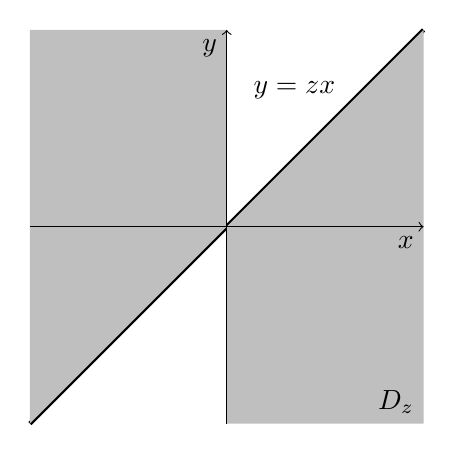
\begin{tikzpicture}[baseline={(current bounding box.north)} ,scale = 0.5]
        \draw [domain=-5:5, smooth, variable = \x, ultra thick] plot ({\x}, 
        {
            \x
        });
        \fill [lightgray, domain=-5:0, smooth, variable = \x] plot ({\x}, 
        {
            \x
        }) -- (0, 5) -- (-5, 5) -- (-5, -5);
        \fill [lightgray, domain=0:5, smooth, variable = \x] plot ({\x}, 
        {
            \x
        }) -- (5, -5) -- (0, -5) -- (0, 0);
        \draw [->] (-5, 0) -- (5, 0);
        \draw [->] (0, -5) -- (0, 5);
        \node [below left] at (5, 0) {$x$};
        \node [below left] at (0, 5) {$y$};
        \node [above left] at (5, -5) {$D_z$};
        \node [above left] at (3, 3) {$y = zx$};
    \end{tikzpicture} &
    \underline{$z > 0$ : }

    $x > 0$ : $y < zx$
    
    $x < 0$ : $y > zx$

    $F_\eta(z) = \int\limits_{-\infty}^0 dx \int\limits_{zx}^{+\infty}f_{\vec{\xi}}(x, y)dy 
    + \int\limits_0^{+\infty}dx\int\limits_{-\infty}^{zx}f_{\vec{\xi}}(x, y)dy$

    Продиференціюємо обидві частини по $z$:

    $f_\eta(z) = -\int\limits_{-\infty}^0 x f_{\vec{\xi}}(x, zx) dx + \int\limits_0^{+\infty}
    xf_{\vec{\xi}}(x, zx)dx$
\end{tabular}

\item 
\begin{tabular}{c p{8.8cm}}
    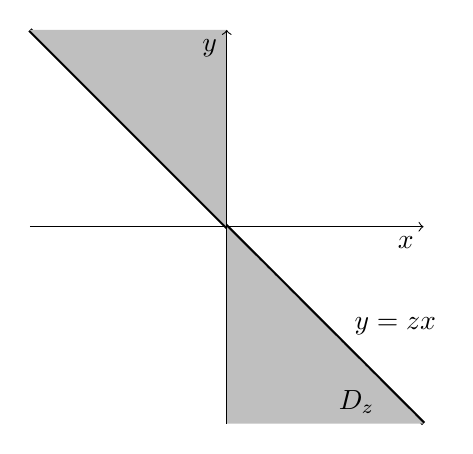
\begin{tikzpicture}[baseline={(current bounding box.north)} ,scale = 0.5]
        \draw [domain=-5:5, smooth, variable = \x, ultra thick] plot ({\x}, 
        {
            -\x
        });
        \fill [lightgray, domain=-5:0, smooth, variable = \x] plot ({\x}, 
        {
            -\x
        }) -- (0, 5) -- (-5, 5);
        \fill [lightgray, domain=0:5, smooth, variable = \x] plot ({\x}, 
        {
            -\x
        }) -- (0, -5) -- (0, 0);
        \draw [->] (-5, 0) -- (5, 0);
        \draw [->] (0, -5) -- (0, 5);
        \node [below left] at (5, 0) {$x$};
        \node [below left] at (0, 5) {$y$};
        \node [above left] at (4, -5) {$D_z$};
        \node [above right] at (3, -3) {$y = zx$};
    \end{tikzpicture} &
    \underline{$z < 0$ : }

    $x > 0$ : $y < zx$
    
    $x < 0$ : $y > zx$

    $F_\eta(z) = \int\limits_{-\infty}^0 dx \int\limits_{zx}^{+\infty}f_{\vec{\xi}}(x, y) dy +
    \int\limits_0^{+\infty}dx\int\limits_{-\infty}^{zx}f_{\vec{\xi}}(x, y)dy $

    Продиференціюємо обидві частини по $z$:

    $f_\eta(z) = -\int\limits_{-\infty}^0 x f_{\vec{\xi}}(x, zx)dy + \int\limits_0^{+\infty}
    xf_{\vec{\xi}}(x, zx)dy$
\end{tabular}
\end{enumerate}

\begin{remark}
    Якщо вказано, що $\xi_1$ та $\xi_2$ --- незалежні, то $f_{\vec{\xi}}(x, zx) = 
    f_{\xi_1}(x)f_{\xi_2}(zx)$.
\end{remark}

\noindent\textbf{Задача 2}: знайти розподіл $\eta = \frac{\xi_1}{\xi_2}$.

Розпишемо функцію розподілу за вже відомою схемою:

$F_\eta(z) = \iint\limits_{D_z}f_{\xi_1\xi_2}(x, y)dxdy$, $D_z = \left\{(x, y)^T \in 
\mathbb{R}^2 : \frac{x}{y} < z\right\}$

\begin{enumerate}[label=\Roman*)]
    \item 
\begin{tabular}{c p{8.8cm}}
    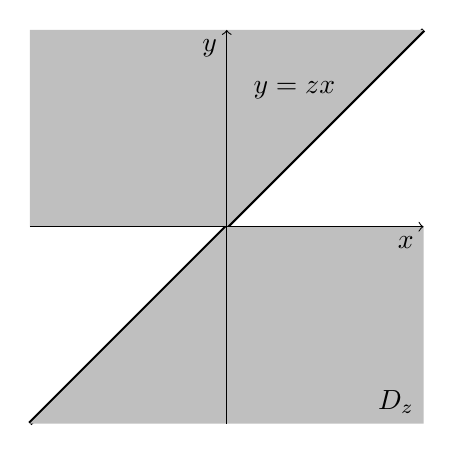
\begin{tikzpicture}[baseline={(current bounding box.north)} ,scale = 0.5]
        \draw [domain=-5:5, smooth, variable = \x, ultra thick] plot ({\x}, 
        {
            \x
        });
        \fill [lightgray, domain=-5:0, smooth, variable = \x] plot ({\x}, 
        {
            \x
        }) -- (5, 0) -- (5, -5) -- (-5, -5);
        \fill [lightgray, domain=0:5, smooth, variable = \x] plot ({\x}, 
        {
            \x
        }) -- (-5, 5) -- (-5, 0) -- (0, 0);
        \draw [->] (-5, 0) -- (5, 0);
        \draw [->] (0, -5) -- (0, 5);
        \node [below left] at (5, 0) {$x$};
        \node [below left] at (0, 5) {$y$};
        \node [above left] at (5, -5) {$D_z$};
        \node [above left] at (3, 3) {$y = zx$};
    \end{tikzpicture} &
    \underline{$z > 0$ : }

    $y > 0$ : $x < zy$
    
    $y < 0$ : $x > zy$

    $F_\eta(z) = \int\limits_{-\infty}^0 dy \int\limits_{zy}^{+\infty}f_{\vec{\xi}}(x, y)dx 
    + \int\limits_0^{+\infty}dy\int\limits_{-\infty}^{zy}f_{\vec{\xi}}(x, y)dx$

    Продиференціюємо обидві частини по $z$:

    $f_\eta(z) = -\int\limits_{-\infty}^0 y f_{\vec {\xi}}(zy, y) dy + \int\limits_0^{+\infty}
    yf_{\vec{\xi}}(zy, y)dy$
\end{tabular}

\item 
\begin{tabular}{c p{8.8cm}}
    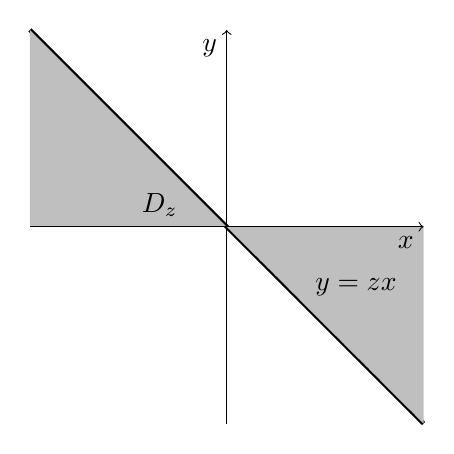
\begin{tikzpicture}[baseline={(current bounding box.north)} ,scale = 0.5]
        \draw [domain=-5:5, smooth, variable = \x, ultra thick] plot ({\x}, 
        {
            -\x
        });
        \fill [lightgray, domain=-5:0, smooth, variable = \x] plot ({\x}, 
        {
            -\x
        }) -- (-5, 0) -- (-5, 5);
        \fill [lightgray, domain=0:5, smooth, variable = \x] plot ({\x}, 
        {
            -\x
        }) -- (5, 0) -- (0, 0);
        \draw [->] (-5, 0) -- (5, 0);
        \draw [->] (0, -5) -- (0, 5);
        \node [below left] at (5, 0) {$x$};
        \node [below left] at (0, 5) {$y$};
        \node [above left] at (-1, 0) {$D_z$};
        \node [above right] at (2, -2) {$y = zx$};
    \end{tikzpicture} &
    \underline{$z < 0$ : }

    $x > 0$ : $y < zx$
    
    $x < 0$ : $y > zx$

    $F_\eta(z) = \int\limits_{-\infty}^0 dy \int\limits_{zy}^{+\infty}f_{\vec{\xi}}(x, y) dx +
    \int\limits_0^{+\infty}dy\int\limits_{-\infty}^{zy}f_{\vec{\xi}}(x, y)dx $

    Продиференціюємо обидві частини по $z$:

    $f_\eta(z) = -\int\limits_{-\infty}^0 y f_{\vec{\xi}}(zy, y)dy + \int\limits_0^{+\infty}
    yf_{\vec{\xi}}(zy, y)dy$
\end{tabular}

\end{enumerate}

\begin{remark}
    Якщо вказано, що $\xi_1$ та $\xi_2$ --- незалежні, то $f_{\vec{\xi}}(zy, y) = 
    f_{\xi_1}(zy)f_{\xi_2}(y)$.
\end{remark}

\subsection{Закон розподілу суми двох НВВ}

Нехай маємо $\vec{\xi} = (\xi_1, \xi_2)^T$ --- неперервний випадковий вектор та
$f_{\xi_1 \xi_2}(x, y)$ відома.

\noindent\textbf{Задача}: знайти розподіл $\eta = \xi_1 + \xi_2$.

Розпишемо функцію розподілу за вже відомою схемою:

$F_\eta(z) = \iint\limits_{D_z}f_{\xi_1\xi_2}(x, y)dxdy$, $D_z = \left\{(x, y)^T \in 
\mathbb{R}^2 : x + y < z\right\}$

\begin{tabular}{c p{8.8cm}}
    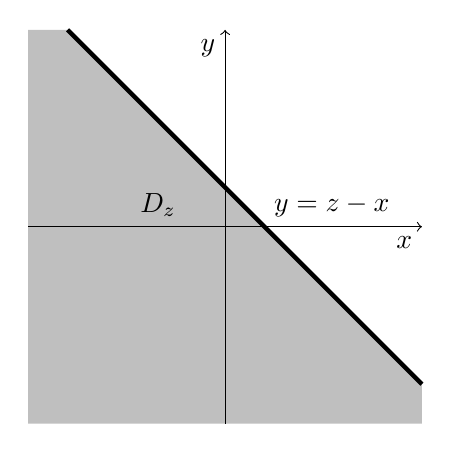
\begin{tikzpicture}[baseline={(current bounding box.north)} ,scale = 0.5]
        \fill [lightgray, domain=-5:5, smooth, variable = \x] 
        (-4, 5) -- (5, -4) -- (5, -5) -- (-5, -5) -- (-5, 5) -- (-4, 5);
        \draw [domain=-4:5, smooth, variable = \x, ultra thick] plot ({\x}, 
        {
            1 - \x
        });
        \draw [->] (-5, 0) -- (5, 0);
        \draw [->] (0, -5) -- (0, 5);
        \node [below left] at (5, 0) {$x$};
        \node [below left] at (0, 5) {$y$};
        \node [above left] at (-1, 0) {$D_z$};
        \node [above right] at (1, 0) {$y = z - x$};
    \end{tikzpicture} &

    $F_\eta(z) = \int\limits_{-\infty}^{+\infty} dx \int\limits_{-\infty}^{z-x} 
    f_{\vec{\xi}}(x, y) dy$

    Продиференціюємо обидві частини по $z$:

    $f_\eta(z) = \int\limits_{-\infty}^{+\infty} f_{\vec{\xi}}(x, z-x) dx$
\end{tabular}

\begin{remark}
    Якщо вказано, що $\xi_1$ та $\xi_2$ --- незалежні, то $f_\eta (z) = 
    \int\limits_{-\infty}^{+\infty}f_{\xi_1}(x) f_{\xi_2}(z-x) dx = 
    (f_{\xi_1} \ast f_{\xi_2})(z)$.
\end{remark}